%\title{Two column article template by M.A.}

\documentclass[11pt, twocolumn]{article}

\usepackage{authblk}

\makeatletter
\renewcommand{\maketitle}{\bgroup\setlength{\parindent}{0pt}
\begin{flushleft}
  \textbf{\@title}

  \@author
\end{flushleft}\egroup
}
\makeatother

\title{\Huge Αλγόριθμος Pagerank με παράλληλη υλοποίηση της μεθόδου Gauss-Seidel \vspace{0.5cm}}
\author{\Large Νικόλαος Κατωμέρης \hspace{2cm} ΑΕΜ: 8551 \hspace{2cm} ngkatomer@auth.gr\normalsize \\ Παράλληλα και διανεμημένα συστήματα. \\Τμήμα ηλεκτρολόγων μηχανικών και μηχανικών υπολογιστών, ΑΠΘ}


\date{\today}

\usepackage[showframe=false, margin=.75in]{geometry}

\usepackage{polyglossia}
\newfontfamily\greekfontsf[Script=Greek]{texgyreheros-regular.otf}
\newfontfamily\greekfonttt[Script=Greek]{Latin Modern Mono}
\setdefaultlanguage{greek}
\setotherlanguage{english}
\setmainfont{Noto Serif}

\usepackage{amsmath}
\usepackage{bm}
\usepackage{abstract}
\renewcommand{\abstractname}{}    % clear the title
\renewcommand{\absnamepos}{empty} % originally center

\usepackage{lipsum}
\usepackage{enumitem}
\usepackage{afterpage}

\renewenvironment{abstract}
 {\small
  \begin{center}
  \bfseries \abstractname\vspace{-.5em}\vspace{0pt}
  \end{center}
  \list{}{%
    \setlength{\leftmargin}{10mm}% <---------- Change margin here
    \setlength{\rightmargin}{\leftmargin}%
  }%
  \item\relax}
 {\endlist}

\usepackage[utf8]{inputenc}
%\usepackage{graphicx}
\usepackage{wrapfig}
\usepackage[lofdepth,lotdepth]{subfig}
\usepackage{booktabs}

\usepackage{titlesec}
\titlespacing\section{0pt}{10pt plus 4pt minus 2pt}{0pt plus 2pt minus 2pt}

\usepackage{rotating}

\usepackage{caption}
%\usepackage{subcaption}

%\usepackage[ngerman]{babel}

\usepackage{csquotes}

\usepackage{todonotes}

\usepackage{stfloats}

%\usepackage[T1]{fontenc}
\usepackage{textcomp}
\usepackage{times}

\usepackage{framed} %um Boxen zu machen

\usepackage[backend=biber, style=ieee]{biblatex}
\addbibresource{references.bib}

%\renewbibmacro*{volume+number+eid}{%
%\printfield{volume}%
%  \setunit*{\adddot}% DELETED
%\setunit*{\addnbspace}% NEW (optional); there's also \addnbthinspace
%\printfield{number}%
%\setunit{\addcomma\space}%
%\printfield{eid}}
%\DeclareFieldFormat[article]{number}{\mkbibparens{#1}}


\usepackage{setspace}
\onehalfspacing

\setlength{\columnsep}{0.8cm}

\setlength{\parskip}{0em}

\usepackage{color}
\definecolor{black}{gray}{0} % 10% gray

\usepackage[colorlinks=true,linkcolor=black,citecolor=black]{hyperref}

\usepackage{tabularx}
\newcolumntype{b}{X}
\newcolumntype{s}{>{\hsize=.5\hsize}X}

\usepackage{ntheorem}
\newtheorem*{TRQ}{Research Question}

\newtheorem{Hyp}{Hypothesis} 


\begin{document}

\twocolumn[
\begin{@twocolumnfalse}
\maketitle
\begin{abstract}
%\textit{\lipsum[2]
%\bigskip}
Στην παρούσα αναφορά περιγράφεται η διαδικασία υλοποίησης και παραλληλοποίησης του αλγορίθμου Gauss-Seidel για τον υπολογισμό του διανύσματος Pagerank ενός γράφου. Επίσης, παρουσιάζονται αποτελέσματα της εκτέλεσης των υλοποιήσεων σε έναν ενδεικτικό γράφο. Για τον κώδικα που αναπτύχθηκε ανατρέξτε στην τελευταία ενότητα.
\end{abstract}
\end{@twocolumnfalse}
]

\section*{Pagerank}
Η βασική ιδέα του αλγορίθμου Pagerank είναι η αξιολόγηση της κάθε σελίδας του διαδικτύου με βάση τον αριθμό των συνδέσμων προς αυτήν και την ποιότητα αυτών, η οποία καθορίζεται από την αξιολόγηση των σελίδων που τους περιέχουν.

Το αποτέλεσμα της παραπάνω αξιολόγησης ταυτίζεται με το ποσοστό του χρόνου στον οποίο ένας τυχαίος περιπατητής θα βρισκόταν στην εκάστοτε σελίδα, αν ξεκινώντας από κάποια τυχαία σελίδα, ακολουθούσε τυχαία κάποιον από τους συνδέσμους της, μετά το ίδιο για την επόμενη κι ούτω καθ' εξής.

Η παραπάνω διαδικασία μπορεί να προσομοιωθεί με μία αλυσίδα Markov της οποίας ο πίνακας μεταβάσεων αποτελείται από στοιχεία που δείχνουν την πιθανότητα μετάβασης από μία σελίδα σε μία άλλη.

Έστω $\bm{A}$, ο $N\times N$  πίνακας μεταβάσεων της αλυσίδας για $N$ σελίδες του διαδικτύου. Αν  $ j\rightarrow i$ σημαίνει ότι η σελίδα $j$ περιέχει σύνδεσμο προς τη σελίδα $i$, ο $\bm{A}$ ορίζεται αρχικά ως εξής:

\[
  \bm{A}(i, j) = 
  \begin{cases}
    1, & \text{αν } j\rightarrow i \\
    0, & \text{αλλιώς }
  \end{cases}
\]

Επειδή όμως ο παραπάνω πίνακας θέλουμε να εκφράζει την πιθανότητα ο περιπατητής να πάει από τη σελίδα $j$ στη σελίδα $i$ σε ένα βήμα, είναι απαραίτητο το άθροισμα των στοιχείων κάθε στήλης του πίνακα να ισούται με $1$.

Οπότε, αφού λάβουμε τον πίνακα με τους συνδέσμους των σελίδων, διαιρούμε όλα του τα στοιχεία με το άθροισμα των στοιχείων της εκάστοτε στήλης $j$, έστω $L_j$, και παίρνουμε τον «στοχαστικοποιημένο» πίνακα $\bm{A}_s$:

\[
  \bm{A}_s(i, j) = 
  \begin{cases}
    \frac{1}{L_j}, & \text{αν } j\rightarrow i \\
    0, & \text{αλλιώς }
  \end{cases}
\]

Επιπλέον, καθώς ο περιπατητής ξεκινά από μία σελίδα, είναι πολύ πιθανό, ακολουθώντας συνεχώς συνδέσμους να είναι αδύνατο να μεταβεί σε όλες τις σελίδες του γράφου. Το γεγονός αυτό, συν το γεγονός ότι ένας χρήστης του διαδικτύου δεν ακολουθεί μόνο συνδέσμους, αλλά «τηλεμεταφέρεται» κιόλας σε άλλες σελίδες, καθιστά τον παραπάνω πίνακα ανεπαρκή για την προσομοίωση της τυχαίας διαδρομής ενός χρήστη του διαδικτύου.

Έτσι, εισάγεται στον αλγόριθμο μια σταθερά «τηλεμεταφοράς» που δηλώνει την πιθανότητα ο περιπατητής να μεταβεί σε κάποια τυχαία σελίδα του διαδικτύου χωρίς να υπάρχει κάποιος σύνδεσμος προς αυτήν στη σελίδα που βρίσκεται.

Η σταθερά αυτή, έστω $c$, μπορεί να επιλεγεί ως όρισμα στο πρόγραμμα υπολογισμού του διανύσματος pagerank που υλοποιήθηκε. Στην περίπτωση που δεν δοθεί, θα έχει την τιμή 0.15 που έχει δειχθεί ότι αποτελεί καλή επιλογή \parencite{brin1998anatomy}.

Με την εισαγωγή της παραπάνω σταθεράς, ο πίνακας μεταβάσεων πλέον θα είναι:
\[
  \bm{A}_{final} = \frac{c}{N}\cdot\bm{1}_{N\times N}+(1-c)\bm{A}_s
\]

Στην παραπάνω σχέση, η σταθερά $c$ διαιρείται με τον αριθμό των γραμμών $N$ έτσι ώστε οι στήλες και του τελικού πίνακα $\bm{A}_{final}$ να έχουν στοιχεία με άθροισμα $1$.

Με τη χρήση του παραπάνω πίνακα είναι δυνατό να υπολογιστεί ένα διάνυσμα $N\times1$ πολλαπλασιάζοντάς τον πίνακα με ένα αρχικό διάνυσμα -πχ ένα ομοιόμορφο- αρκετές φορές, έως ότου το αποτέλεσμα συγκλίνει. Το διάνυσμα αυτό αποτελεί ιδιοδιάνυσμα του πίνακα $\bm{A}$ για την ιδιοτιμή 1 και αποτελεί το ζητούμενο διάνυσμα με την αξιολόγηση της κάθε σελίδας (κόμβου).

Για να συγκλίνει με βεβαιότητα το διάνυσμα απαιτείται ακόμη ένα βήμα, θα πρέπει, αν ο περιπατητής βρεθεί σε κάποια σελίδα που δεν περιέχει καμία σύνδεση, να τηλεμεταφερθεί σε μία τυχαία σελίδα με βάση ένα διάνυσμα πιθανοτήτων. Στην υλοποίηση αυτή, ο περιπατητής έχει την ίδια πιθανότητα να τηλεμεταφερθεί σε οποιαδήποτε σελίδα.

Με όλα τα παραπάνω δεδομένα, αποδεικνύεται ότι ο τελικός πίνακας θα έχει μία ιδιοτιμή ένα και το πρόβλημα πλέον έγκειται στην εύρεση του ιδιοδιανύσματός της.

Για την εύρεση του ιδιοδιανύσματος, όπως ζητείται, χρησιμοποιείται η μέθοδος Gauss-Seidel.



\section*{Gauss Seidel}
H μέθοδος Gauss-Seidel είναι μια αναδρομική μέθοδος επίλυσης γραμμικών συστημάτων. Ο αναδρομικός αλγόριθμός της μεθόδου για την επίλυση ενός γραμμικού συστήματος της μορφής:
$$\bm{A}\vec{x}=\vec{b}$$
είναι για το $i$-στο στοιχείο στο $k+1$ βήμα:
$$x_i(k+1) = \frac{1}{A_{ii}}\bigg(b_i-\sum_{j=1}^{i-1}A_{ij}x_j(k+1)-\sum_{j=i+1}^{N}A_{ij}x_j(k)\bigg)$$

Όπως φαίνεται, ο αλγόριθμος αυτός μοιάζει καθαρά σειριακός αφού ο υπολογισμός του κάθε στοιχείου σε κάθε βήμα εξαρτάται από τον υπολογισμό των νέων τιμών των στοιχείων πριν απ' αυτό.
Για περισσότερες λεπτομέρειες σχετικά με τη μέθοδο αυτή και τα κριτήρια σύγκλισής της ανατρέξτε στον \textcite{saad2003iterative}.

Στην περίπτωσή μας, για την εύρεση της pagerank με τη μέθοδο Gauss-Seidel, θα πρέπει πρώτα να το εκφράσουμε σαν σύστημα γραμμικών εξισώσεων. Όπως προαναφέρθηκε το διάνυσμα Pagerank αποτελεί ιδιοδιάνυσμα του πίνακα $\bm{A}$ για την ιδιοτιμή 1. Επομένως, ισχύει ότι:\\
\begin{multline*}
\bm{A}_{final}\vec{x} = \vec{x}\Rightarrow (\bm{I}-\bm{A}_{final})\vec{x} = 0 
\Rightarrow \\
\bigg(\bm{I}-\frac{c}{N}\cdot\bm{1}_{N\times N}-(1-c)\bm{A}_n\bigg)\vec{x} = 0
\end{multline*}

Όμως, το $\bm{1}_{N\times N}\cdot\vec{x}$ είναι πάντα ίσο με $\bm{1}_{N\times1}$ επειδή το άθροισμα των στοιχείων του $\vec{x}$, ως άθροισμα όλων των πιθανοτήτων, εκφράζει την πιθανότητα ο περιπατητής να βρίσκεται σε μια οποιαδήποτε σελίδα.
 Έτσι, το σύστημά μας παίρνει τη μορφή:

\begin{equation} \label{eq:1}
(\bm{I}-(1-c)\bm{A}_n)\vec{x} = \frac{c}{N}\bm{1}_{N\times1}
\end{equation}

που μπορεί να λυθεί αναδρομικά με τη μέθοδο Gauss-Seidel, αρκεί διασφαλιστεί ότι σε κάθε βήμα $\bm{1}_{N\times N}\cdot\vec{x}_k =\bm{1}_{N\times1}$, δηλαδή ότι το άθροισμα των στοιχείων του $\vec{x}_k$ παραμένει ένα.


\section*{Δεδομένα στη μνήμη}
Το πρόβλημα με την \fref{eq:1} είναι ότι ο πίνακας $(\bm{I}-(1-c)\bm{A}_n)$ δεν είναι αραιός καθώς ο $\bm{A}_n$ , όπως αναφέρθηκε νωρίτερα, έχει γεμάτες τις στήλες με τις σελίδες που στον $\bm{A}_s$ δεν είχαν καμία σύνδεση. Επίσης, το σύνολο αυτών των σελίδων στο διαδίκτυο είναι πολύ μεγάλο\parencite{eiron2004ranking}, με αποτέλεσμα ο $\bm{A}_n$ να απαιτεί πολύ περισσότερο χώρο στη μνήμη από τον $\bm{A}_s$.

Έχουν προταθεί διάφορες λύσεις για την αποφυγή αυτού του φαινομένου, όπως για παράδειγμα να προστεθεί σ' όλες αυτές τις σελίδες σύνδεσμος προς τον εαυτό τους. Μια άλλη πρόταση, η οποία και προτιμήθηκε, χρησιμοποιεί μόνο τον πίνακα $\bm{A}_s$ ο οποίος είναι αραιός και καταλήγει στην ίδια ακριβώς λύση με την \fref{eq:1}. Όπως αποδεικνύεται \parencite{del2005fast}, η λύση της \fref{eq:1} ισοδυναμεί με $\frac{\vec{y}}{\Vert\vec{y}\Vert}_1$, όπου $\vec{y}$ η λύση της:
\begin{equation}\label{eq:2}
(\bm{I}-(1-c)\bm{A}_s)\vec{y} = \frac{1}{N}\cdot\bm{1}_{N\times1}
\end{equation}

H οποία απαιτεί την αποθήκευση μόνο του πίνακα $\bm{A}_s$. Δεδομένου ότι ο πίνακας αυτός είναι πολύ αραιός, αλλά και λόγω του γεγονότος ότι η μέθοδος gauss-seidel έχει, σε κάθε της βήμα και για κάθε κόμβο, πολλαπλασιασμούς στοιχείων μίας γραμμής του $\bm{A}_s$, επιλέχθηκε η χρήση της δομής «Compressed Row Storage (CRS)». 

Η δομή αυτή επιτρέπει την αποθήκευση πινάκων σε χώρο στη μνήμη ανάλογο με τα μη μηδενικά στοιχεία αυτών. Επιπλέον, διατρέχοντας τον πίνακα ανά γραμμή, όλα τα στοιχεία της γραμμής βρίσκονται συνεχόμενα στη μνήμη καθιστώντας τη δομή αυτή φιλική προς την μνήμη cache των επεξεργαστών.

\section*{Σειριακός αλγόριθμος}
Με βάση τα παραπάνω, υλοποιήθηκε το σειριακό πρόγραμμα υπολογισμού της pagerank. Συνοψίζεται ως εξής:
\begin{enumerate}

\item Επιλογή γράφου δεδομένων εισόδου (σύνδεσμοι) και προαιρετικά συγκεκριμένου αριθμού επαναλήψεων ή σταθερών τηλεμεταφοράς ($c$) και σύγκλισης ($E$). Οι προεπιλεγμένες τιμές είναι: \\ $c_{def} = 0.15, E_{def} = 1e-12$

\item Φόρτωση στη μνήμη των δεδομένων εισόδου σε δομή CRS. Tα δεδομένα αυτά αποτελούν τον αρχικό πίνακα $\bm{A}$.

\item Μετατροπή του $\bm{A}$ στον $\bm{A}_s$ και πολλαπλασιασμός του με την σταθερά $-(1-c)$. Έστω $a_{ij}$ τα στοιχεία του πίνακα που προκύπτει.

\item Δημιουργία των $\vec{b},\vec{x}_0=\frac{1}{N}\bm{1}_{N\times1}$

\item Εκτέλεση αναδρομικού αλγορίθμου της μεθόδου Gauss-Seidel έως ότου $\Vert\vec{x}_{k+1}-\vec{x}_k\Vert^2 < E$ ή $k > k_{max}$, όπου έχει προκαθοριστεί $k_{max} = 150$ για ασφάλεια. Επίσης, αν έχει δοθεί συγκεκριμένος αριθμός επαναλήψεων, θα χρησιμοποιηθεί αυτός.

Σε κάθε βήμα του αλγορίθμου:
\begin{itemize}[leftmargin=*]
\item Yπολογίζεται το $x_{k+1}$:

\hfil$\displaystyle x_i(k+1) = \frac{1}{1-a_{ii}}\bigg(b_i-\sum_{j=1}^{i-1}a_{ij}x_j(k+1)-\sum_{j=i+1}^{N}a_{ij}x_j(k)\bigg)$\hfil

\item Κάθε στοιχείο $x_{k+1}$ διαιρείται με το άθροισμα όλων των στοιχείων του, ώστε το νέο $x_{k+1}$ να ισχύει η προϋπόθεση ότι το άθροισμα των στοιχείων του $x$ σε κάθε βήμα πρέπει να ισούται με 1.

\item Υπολογίζεται το $\Vert\vec{x}_{k+1}-\vec{x}_k\Vert^2$ και αυξάνεται το $k$ κατά 1.

\end{itemize}
\end{enumerate}

\section*{Παραλληλοποίηση}
Η μέθοδος gauss-seidel γενικώς είναι μια σειριακή μέθοδος. Σε περιπτώσεις όμως που ο πίνακας $\bm{A}$ είναι αραιός, όπως και στην προκειμένη, είναι δυνατός ο παράλληλος υπολογισμός των $x_i$ που δεν αλληλοεξαρτώνται και εξαρτώνται μόνο από στοιχεία $x_j\text{με } j < i$, των οποίων η τιμή έχει ήδη ενημερωθεί, ή στοιχεία που δεν χρειάζεται να έχουν ενημερωθεί ($j > i$).

Για την εύρεση των ομάδων αυτών με τα μη αλληλοεξαρτώμενα στοιχεία του $x$ υλοποιήθηκε ο εξής άπληστος αλγόριθμος:

\begin{itemize}
\item Διατρέχουμε κατά αύξουσα σειρά τα στοιχεία (κόμβους) του γράφου.
\item Τον 1ο κόμβο τον εισάγουμε στην 1η ομάδα.
\item Tον 2ο κόμβο τον εισάγουμε κι αυτόν στην 1η ομάδα εκτός αν υπάρχει σύνδεσμος μεταξύ αυτού και του 1ου. Σε εκείνη την περίπτωση τον τοποθετούμε στην 2η ομάδα.
\item Συνεχίζουμε με τους υπόλοιπους κόμβους, τοποθετώντας τους κάθε φορά στην Λ+1 ομάδα όπου Λ η μεγαλύτερη ομάδα των κόμβων που συνδέονται μ' αυτούς.
\end{itemize}

Αφού, γίνει ο ο «χρωματισμός» των κόμβων σε ομάδες προχωράμε σε ανακατάταξη των κόμβων έτσι ώστε τα στοιχεία της κάθε ομάδας να βρίσκονται συνεχόμενα στη μνήμη και με αύξουσα σειρά ομάδας.

Ύστερα, η εύρεση του διανύσματος pagerank είναι όμοια με τον σειριακό αλγόριθμο με τη διαφορά ότι εδώ υπολογίζουμε παράλληλα τις τιμές $\vec{x}_i(k+1)$ σε κάθε βήμα για τα $i$ που βρίσκονται στην ίδια ομάδα. Επίσης, παράλληλα γίνονται και όλες οι πράξεις πινάκων που απαιτούνται για τον έλεγχο σύγκλισης.

Τέλος, οι κόμβοι επιστρέφουν στην αρχική τους αλληλουχία ώστε να γίνει εύκολα σύγκριση του αποτελέσματος με τον σειριακό αλγόριθμο.


\section*{Συνθήκες και περιορισμοί}
\begin{itemize}[leftmargin=*]
\item Η διαθέσιμη μνήμη του συστήματος περιορίζει το μέγιστο όριο κόμβων/συνδέσμων που μπορούν να εισαχθούν στο πρόβλημα. Αυτό το όριο περιορίζεται και από τη χρήση 32-bit μεταβλητών για τους κόμβους. Δηλαδή, δεν μπορούν να χρησιμοποιηθούν γράφοι με πάνω από περίπου 4.3δις κόμβους.
\item Τα αρχεία με τους συνδέσμους που επιλέγονται ως είσοδος στα προγράμματα υπολογισμού της pagerank, πρέπει να είναι συγκεκριμένης μορφής για να είναι συμβατά.

Στα παραδοτέα, συμπεριλαμβάνεται ειδικό πρόγραμμα που μετατρέπει αρχεία κειμένου σαν αυτά των \textcite{snapnets} σε συμβατά αρχεία για τα προγράμματα υπολογισμού της pagerank. Το πρόγραμμα αυτό, διαβάζει στην έναρξη των αρχείων τον συνολικό αριθμό κόμβων και απορρίπτει κάθε κόμβο με id μεγαλύτερο αυτού του αριθμού.

\item Η παραλληλοποίηση των iteration της μεθόδου gauss-seidel γίνεται μόνο στις ομάδες που περιέχουν περισσότερους από 50 κόμβους, καθώς το overhead της παραλληλοποίησης κάνει την παράλληλη εκτέλεση του αλγορίθμου μη αποδοτική για μικρότερες ομάδες. Αυτός ο αριθμός, μπορεί εύκολα να αλλάξει ώστε να ταιριάζει στο εκάστοτε σύστημα.

\item Σε ορισμένα web-graphs, στα οποία ο αριθμός των ομάδων που προκύπτει με τον greedy αλγόριθμό είναι αρκετά μεγάλος, ο σειριακός αλγόριθμος θα είναι πιθανότατα ταχύτερος. Χρήση διαφορετικής, αλληλουχίας των κόμβων θα δώσει διαφορετικά αποτελέσματα τόσο στη σύγκλιση όσο και στον αριθμό των διαφορετικών ομάδων.

\item Δεν επιχειρήθηκε αναζήτηση ακολουθίας κόμβων που θα οδηγούσε σε ταχύτερη σύγκλιση ή καλύτερη διαχωρισιμότητα για την παράλληλη υλοποίηση. Όλοι οι κόμβοι διαβάζονται όπως βρίσκονται στο αρχείο και η παραλληλοποίηση γίνεται με τρόπο που δεν επηρεάζει τη σύγκλιση.

\item Τόσο η σειριακή όσο και η παράλληλη υλοποίηση, εκτός των αποτελεσμάτων, δημιουργούν σε κάθε τους εκτέλεση κι ένα αρχείο με δεδομένα χρόνων ή κι άλλα χρήσιμα δεδομένα. Τα διαγράμματα που παρουσιάζονται στην επόμενη ενότητα συγκρίνουν τους καθαρούς χρόνους εκτέλεσης του αλγορίθμου Pagerank των δυο υλοποιήσεων, δηλαδή δεν αφορούν τον απόλυτο χρόνο εκτέλεσης του κάθε προγράμματος.
\end{itemize}




\section*{Ενδεικτικά αποτελέσματα}
Έγινε εκτέλεση των δύο υλοποιήσεων στα web graphs των \textcite{snapnets}.

Παρακάτω παρουσιάζονται διαγράμματα τα διάφορα χαρακτηριστικά των εκτελέσεων.
\begin{center}
\begin{figure}
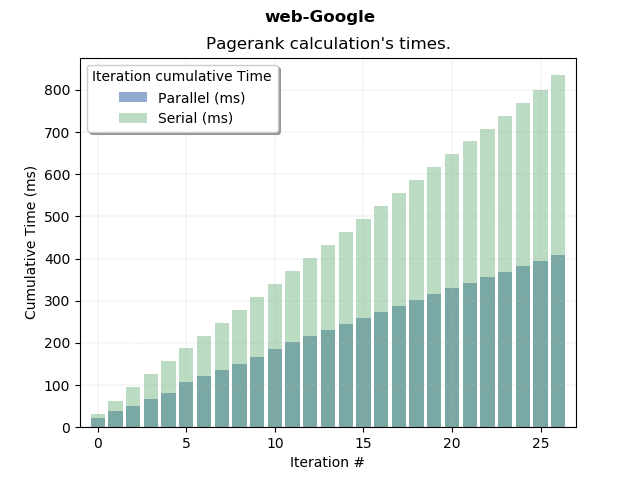
\includegraphics[width=\linewidth]{plots/it_time.png}
\caption{Χρονική εξέλιξη των δύο υλοποιήσεων. 4-πύρηνο σύστημα.}
\end{figure}

\begin{figure}
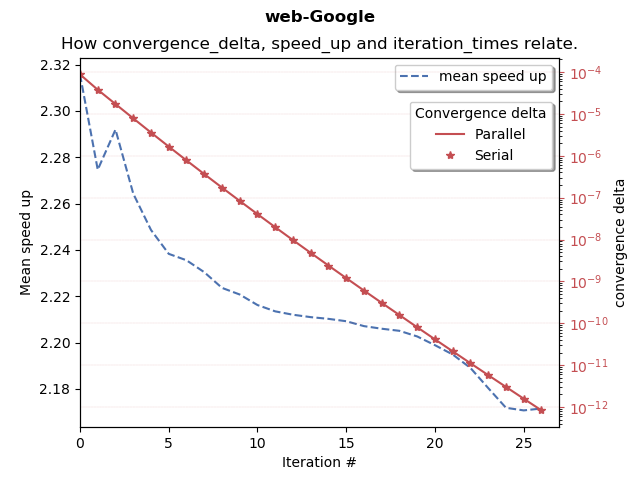
\includegraphics[width=\linewidth]{plots/speed_up.png}
\caption{Σχέση σταθεράς σύγκλισης, επιτάχυνσης και αριθμού επαναλήψεων. 4-πύρηνο σύστημα.}
\end{figure}

\begin{figure}
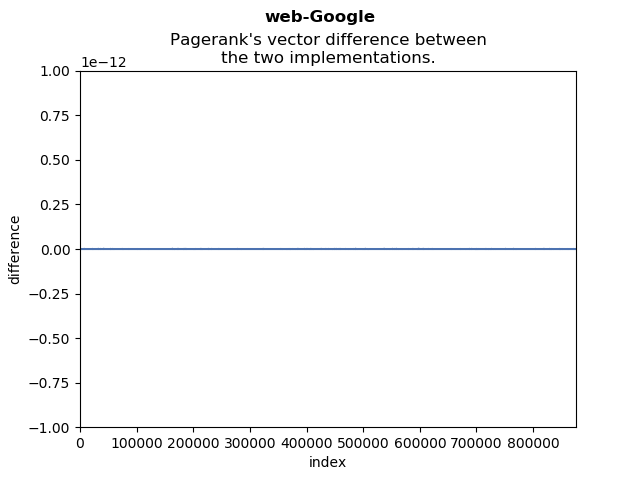
\includegraphics[width=\linewidth]{plots/diff.png}
\caption{Διαφορά των δύο υλοποιήσεων στο τελικό διάνυσμα.}
\end{figure}

\begin{figure}
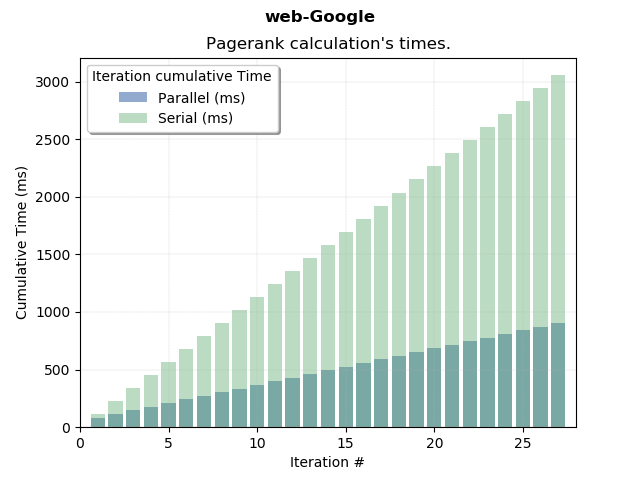
\includegraphics[width=\linewidth]{plots/it_times_diades.png}
\caption{Χρονική εξέλιξη των δύο υλοποιήσεων. 8-πύρηνο σύστημα.}
\end{figure}

\begin{figure}
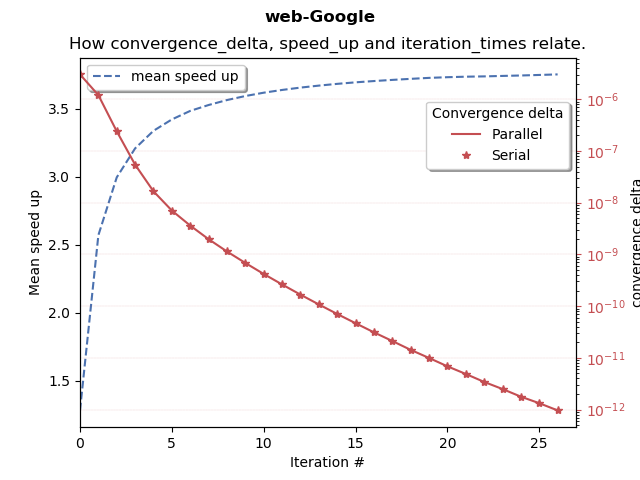
\includegraphics[width=\linewidth]{plots/speed_up_diades.png}
\caption{Σχέση σταθεράς σύγκλισης, επιτάχυνσης και αριθμού επαναλήψεων. 8-πύρηνο σύστημα.}
\end{figure}

\begin{figure}
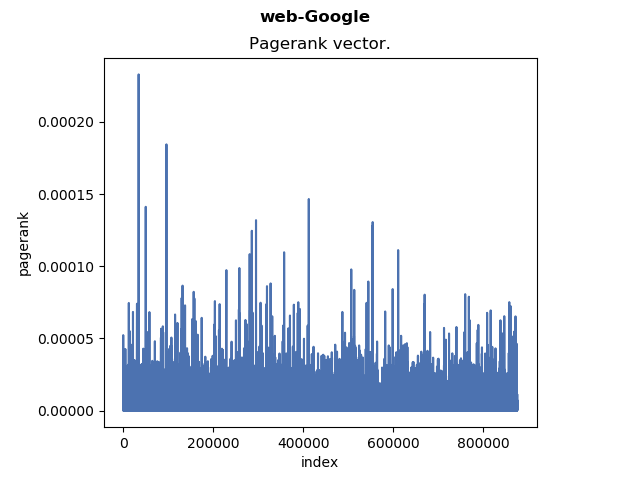
\includegraphics[width=\linewidth]{plots/pagerank.png}
\caption{Το αποτέλεσμα για κάθε κόμβο.}
\end{figure}

\end{center}
Τα web graph που χρησιμοποιήθηκε περιείχε 875.713 κόμβους με 4.563.235 συνδέσμους ενώ δύο συστήματα έχουν τα εξής χαρακτηριστικά: 
\begin{enumerate}

\item 4 πύρηνο σύστημα
\begin{itemize}
\item Intel(R) Core(TM) i5-4670 CPU @ 3.40GHz.
\item 8GB DDR3 RAM
\item gcc version 7.3.0
\end{itemize}

\item 8 πύρηνο σύστημα (diades)
\begin{itemize}
\item Intel(R) Xeon(R) CPU E5420  @ 2.50GHz.
\item 8GB DDR3 RAM
\item gcc version 5.4.0
\end{itemize}
\end{enumerate}

Στα παραδοτέα, περιέχονται έτοιμα τα αποτελέσματα και για τα υπόλοιπα web-graphs. Γενικώς, παρατηρήθηκε ικανοποιητική επιτάχυνση με ταχύτητες έως και 240\% στο τετραπύρηνο ή/και έως 360\% στο οχταπύρηνο σύστημα σε σχέση με τη σειριακή υλοποίηση, για όλα τα δεδομένα με εξαίρεση το web-BerkStan graph όπου ο edge-coloring αλγόριθμος δημιούργησε ιδιαίτερα αυξημένο αριθμό ομάδων. Σε εκείνη την περίπτωση, ο πιο σύγχρονος και γρήγορος επεξεργαστής του 4-πύρηνου συστήματος, εμφάνισε επιτάχυνση έως 120\% περίπου.

Στην παράλληλη υλοποίηση δίνεται και η δυνατότητα επιλογής σταθερού αριθμού threads που θα δημιουργήσει το openMP, η επιλογή αυτή, όμως, οδηγεί συνήθως σε χειρότερη επίδοση του προγράμματος.




\section*{Επαλήθευση ορθότητας αποτελεσμάτων}
Αρχικά, ο αλγόριθμος υπολογισμού της pagerank που υλοποιήθηκε υποστηρίζεται μαθηματικά σε κάθε του βήμα. Σε κάθε περίπτωση, για να αποκλειστεί η πιθανότητα προγραμματιστικού λάθους, έγινε επαλήθευση αποτελεσμάτων για μικρής κλίμακας web-Graphs με προϋπάρχουσες υλοποιήσεις \parencite{mastersthesis} σε γλώσσα προγραμματισμού \textit{MATLAB}. Αυτές οι υλοποιήσεις συμπεριλαμβάνονται στα παραδοτέα, καθώς και τα script που χρησιμοποιήθηκαν για τη σύγκριση των αποτελεσμάτων.

Η ορθότητα του παράλληλου αλγορίθμου μπορεί να επιβεβαιωθεί κι από την ταύτιση των αποτελεσμάτων του με αυτά του σειριακού, όπως φαίνεται στο \fref{fig:dif}. Επιπλέον, έχουν πάντα ακριβώς ίδιο αριθμό από iterations και ίδια ακολουθία σύγκλισης όπως φαίνεται στα \fref{fig:relat} και \fref{fig:relatd}.

Καθώς ο σκοπός της εργασίας ήταν η παραλληλοποίηση του αλγορίθμου, δεν έγινε αλλαγή στην αλληλουχία των κόμβων με τρόπο που θα διαφοροποιούσε το παράλληλο από το σειριακό πρόγραμμα, καθώς η σύγκλιση της μεθόδου gauss-seidel εξαρτάται από αυτή την αλληλουχία. Έτσι, μπορεί να επιβεβαιωθεί η ταύτιση των αποτελεσμάτων των δύο υλοποιήσεων.

Επιπλέον, μπορεί να επιβεβαιωθεί και πειραματικά η απουσία race condition στην παράλληλη υλοποίηση από το γεγονός ότι συγκλίνει πάντα με τον ίδιο τρόπο που ταυτίζεται και μ' αυτόν της σειριακής.

Τέλος, έχει επιβεβαιωθεί (με το εργαλείο valgrind) ότι τα προγράμματα αυτά δεν παρουσιάζουν σφάλματα μνήμης.


\section*{Tαχύτητα σύγκλισης κι εκτέλεσης}
Η ταχύτητα σύγκλισης της μεθόδου gauss-seidel όπως φαίνεται στα αποτελέσματα είναι εντυπωσιακή. Το διάνυσμα της pagerank άρχισε να συγκλίνει από τις πρώτες κι όλας επαναλήψεις, με το τετράγωνο του μέτρου της διαφοράς των τελευταίων προσεγγίσεων να είναι μικρότερο -σε όλες τις περιπτώσεις- του $10^{-5}$ πριν την 7η επανάληψη. 

Αυτός ο   ρυθμός σύγκλισης την καθιστά ταχύτερη τόσο από, την κλασσική για το πρόβλημα, power method\parencite{silvestrepagerank} όσο και από την μέθοδο Jacobi που χρησιμοποιεί μόνο τις προηγούμενες τιμές κάθε $x_i$ σε κάθε επανάληψη.

Η επιτάχυνση της παράλληλης υλοποίησης, λαμβάνοντας υπόψη τις συνθήκες του αλγορίθμου, τον αριθμό των διαφορετικών χρωμάτων και τις επιταχύνσεις που επιτεύχθηκαν στη βιβλιογραφία\parencite{hasenplaugh2016parallel}, κρίνεται κι αυτή από ικανοποιητική έως πάρα πολύ καλή για τα τρία από τα τέσσερα web-graphs στα οποία εξετάστηκε.

\section*{Παραδοτέα}
Το repository με όλα τα αρχεία της εργασίας βρίσκεται
\href{https://github.com/nicktheway/Pagerank}{εδώ}.

Επιπλέον, το documentation του κώδικα σε C της εργασίας βρίσκεται
\href{https://nicktheway.github.io/Pagerank/html/index.html}{εδώ}.

\printbibliography

 
\end{document}
\clearpage
\appendix
\renewcommand\thefigure{A\arabic{figure}}
\setcounter{figure}{0}


\section*{Appendix}

Appendix content


\end{document}
